\chapter{Introduction} % Main chapter title
%\selectlanguage{serbianc}
%\sffamily
%\fontencoding{OT2}\fontfamily{Tempora-TLF}\selectfont

Many real systems, such as brain network, social organizations, cities or even biological systems, can be represented as a complex systems. The common property of these systems is that they are composed of many interacting elements. Still, to describe the properties of the system, we can not conclude too much from the behaviour of a single individual. Due to specific interactions, without any central force, in the complex system emergence, the collective behaviour \cite{kwapien2012}. The structure of the brain network and its properties are fundamental for brain functioning, while an emergent phenomenon is human intelligence. In societies, people's interactions lead to civilization, economy, formation of social groups. Also, the animal populations show different levels of organization: such as bird flocks or schools of fishes \cite{thurner2018}.

An important property of the complex systems is called universality \cite{binney1992}. The empirical analysis showed that universality is characteristic of many collective social phenomena  \cite{chatterjee2013, radicchi2008}. Even the growth of social groups, such as cities, follow universal patterns. The probability distribution of the city sizes in one country follows the same laws, with a similar exponent for all countries \cite{barthelemy2019}. Understanding how universalities in the system emerge is the focus of statistical physics of complex systems \cite{verbavatz2020}. 

%Emergent collective behavior is an indispensable property of complex systems \cite{ladyman2013}. It occurs as a consequence of interactions between a large number of units that compose a complex system, and it cannot be easily predicted from the knowledge about the behavior of these units. The previous research offers a definite proof that the structure of the interaction network is inextricably associated with dynamic and function of the complex system \cite{barrat2008, pascual2006, castellano2009, gosak2018, arenas2008, boccaletti2016, chen2018, kuga2018}. The structure of complex networks is essential for understanding the evolution and function of various complex systems \cite{boccaletti2006,newman2010, holme2012, boccaletti2014}. 

The research in complex systems focuses on the interactions between its units. The interactions are not homogeneous; as the system evolves, we also find that interactions become specific and nonlinear \cite{thurner2018}. Knowing how units of the system are connected, we can determine the emergence of the collective behaviour of the system \cite{ladyman2013}. For the brain network, we can construct representation with neurons and synapses, representing the brain connectivity. Neurons in the same brain area are closely connected \cite{latora2017complex}.
Similarly, we can define communication between people. The structure of these interactions gives us insights, for example, how information propagates through the system. The presence of people with many connections can lead to faster information flow. 

Despite the differences between complex systems, they can be studied using the same techniques. The natural extension of the complex system is the network, sets of nodes (vertices) and links (edges). Elements in the system are nodes, while interactions between them are given as edges. This approximation allows us to treat equally social \cite{myers2014, sarigol2014} (graph of actors) , biological (network of proteins) \cite{fraiman2009ising, schneider2011modeling} or even technological systems (internet, traffic) \cite{costa2007characterization, costa2011analyzing, newman2003structure}. The complex network theory has applications in different fields, and the availability of big data and great computational efforts incurs its development. 

The complex network theory originates from the graph theory in mathematics. 
The first mathematical problem solved using graph theory was $Konigsberg$ problem of seven bridges. The city $Konigsberg$ had seven bridges connecting the city's parts across the river and the island in the middle. The question was, is it possible to find a walk that crosses all seven bridges only once. Representing the problem as a graph, as in figure \ref{fig:Krgraph}, Euler managed to simplify the problem; the parts of the land are represented as nodes while bridges between them are links. Crossing each bridge only once is possible if each part of the land has an even number of connections. It makes possible to enter one part of the land from one bridge and leave it on the other. As each node has an odd number of connections, in this case, it is not possible; see Fig. \ref{fig:Krgraph}.

\begin{figure}[!ht]
	\centering
	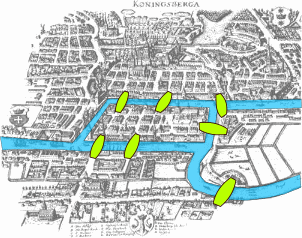
\includegraphics[width=0.3\linewidth]{Konigsberg_bridges.png} \hspace{2cm}
	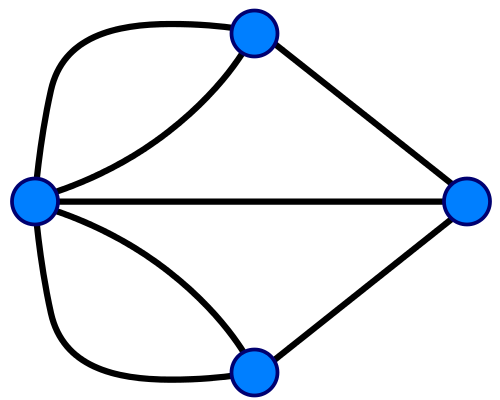
\includegraphics[width=0.3\linewidth]{Konigsberg_graph.png}
	\caption[\selectlanguage{english}Konigsberg problem of seven bridges.]{The Kronigsber problem of seven bridges. The left panel shows the original map of the bridges; the right panel shows its graph representation. }

	\label{fig:Krgraph}
\end{figure}
%TODO review network models
The analysis of different real networks showed that they share common properties \cite{boccaletti2006complex}: small-world behaviour, large clustering and scale-free structure. Small-world property means that the distance between any two nodes is small and scales as logarithmic with the degree of the node. Real systems show high clustering, and the most prominent feature is scale-free property, where the degree distribution follows the power law. In the random network model (Erdős-Rényi) each node has an equal connecting probability, \cite{dorogovtsev2010complex}. This model produces Poisson degree distribution, contrary to those properties observed from data, so it could not describe real systems. Two seminal papers from 1999. by Watts and Strogatz \cite{watts1998collective}, and the Barabási-Albert model \cite{barabasi1999} inspired further research in this field. Watts and Strogatz  \cite{watts1998collective} proposed a new model that could generate networks with small-world properties, while the Barabasi-Albert model generates scale-free networks. 

The combination of network growth and linking rules- new nodes prefer high degree nodes- lead to scale-free degree distribution. Since then, different complex networks models were proposed in order to better describe the dynamics of social and technological systems. As linking probability in the BA model is linear with node degree, first generalization was to introduce nonlinear dependence. Further, the linking probability may depend on the node age \cite{dorogovtsev2000b, dorogovtsev2001b}, or any other feature; fitness. Some models considered that nodes become inactive, or even that network grows through nonlinear number of links \cite{pham2016}. On the other hands were considered models with accelarated growth in the number of nodes \cite{sen2004}, in order to simulated exponential expansion of the online social systems. The empirical analysis of various online social systems show that their growth is time dependent and often accelerated \cite{liu2019}. The number of new nodes joining in time has trends and reflect the typical human behavior \cite{mitrovic2010a, mitrovic2012, mitrovic2015 }. 


%The idea of small world property dates from Milgram, he showed that average path length between individuals is small. This was tested on online social networks by Ugander et al., they showed that users on Facebook were within six degrees of separation. 








%TODO: review sociophysics
\cite{schweitzer2018sociophysics}


%%%%%%%%%%%%%%%%%%%%%%%%%%%%%%%%%%%%%%%%%%%%%%%%%%%%%%%%%%%%%%%%%%

 

%The structure and dynamics of real complex systems are studied using complex network theory \cite{boccaletti2006,newman2010, ladyman2013}. It was shown that real networks have similar topological properties regardless of their origins \cite{barabasi2009}. They have broad degree distribution, degree-degree correlations, and power-law scaling of clustering coefficient \cite{barabasi2009,newman2010}. Understanding how these properties emerge in complex networks leads to the factors that drive their evolution and shape their structure \cite{barrat2008}.

%The complex network models substantially contribute to our understanding of the connection between the network topology and system dynamics and uncover underlying mechanisms that lead to the emergence of distinctive properties in real complex networks \cite{barabasi1999, tadic2001, mitrovic2009}. For instance, the famous Barabasi-Albert model \cite{barabasi1999} finds the emergence of broad degree distribution to be a consequence of preferential attachment and network growth. Degree-degree anti-correlations of the Internet can be explained, at least to a certain extent, by single edge constrain \cite{maslov2004, park2003}. Detailed analysis of emergence of clustered networks shows that clustering is either the result of finite memory of the nodes \cite{klemm2002} or occurs due to triadic closure \cite{serrano2005}. 

%Network growth, in combination with linking rules, shapes the network topology \cite{vazquez2003}. While various rules have been proposed to explain the topology of real networks \cite{boccaletti2006}, most models assume a constant rate of network growth, i.e., the addition of a fixed number of nodes at each time step \cite{barabasi1999, klemm2002, serrano2005}. However, the results of empirical analysis of numerous technological and social systems show that their growth is time-dependent \cite{huberman1999, mitrovic2010a, mitrovic2015, liu2019}. The accelerated growth in complex networks is the cause of the high heterogeneity in the distribution of webpages among websites \cite{huberman1999} and the emergence of highly cited authors in citation networks \cite{liu2019}. The growth of real systems is not always accelerated. The number of new nodes joining the system varies in time, has trends, and exhibits circadian cycles typical for human behavior \cite{mitrovic2010a, mitrovic2012, mitrovic2015}. These signals are multifractal and have long-range correlations \cite{kantelhardt2002}. Some preliminary evidence shows that the time-varying growth influences the structure and dynamics of the social system and, consequently, the structure of interaction networks in social systems \cite{mitrovic2012,mitrovic2011,mitrovic2015,tadic2017,tadic2013}. Still, which properties of the real growth signal have the largest influence, how different properties influence the topology of the generated networks and to what extent is an open question.


%%%%%%%%%%%%%%%%%%%%%%%%%%%%%%%%%%%%%%%%%%%%%%%%%%%%%%%%%%%%%%%%%%%%%%%%%%%%%%%%%%%%%


%The development of a knowledge-based society is one of the critical processes in the modern world \cite{leydesdorff2001sociological,leydesdorff2012triple}. In a knowledge-based society, knowledge is generated, shared, and made available to all members. It is a vital resource. Sharing this resource between individuals and organizations is a necessary process, and knowledge-sharing communities are one of the fundamental elements of a knowledge society.

%Often, these knowledge-sharing communities depend on the willingness of their members to engage in an exchange of information and knowledge. Participation in the community is voluntary, with no noticeable material gains for members. Thus, the exchange of knowledge depends on mutual trust between members. Trust that the community will consider their questions essential for the growth of the knowledge corpus and invest resources to answer their questions. Trust that the community will objectively evaluate their answers based on their quality and clarity. The trust mentioned is beyond the direct trust formed between two members. It is a feeling of a member that a community can be trusted and that their engagement is valuable. A feeling of community that a member can be trusted and expressed through engaging that member in community activities. It is a collective phenomenon that depends on and is built through social interactions between community members. This is why we believe it is crucial to understand how trustworthy knowledge-sharing communities emerge and disappear, as well as to unveil the fundamental mechanisms that underlie their evolution and determine their sustainability.

%In the past two decades, we have witnessed the emergence of an online knowledge-sharing community StackOverflow, which has become one of the most popular sites in the world and the primary knowledge resource for coding. The success of StackOverflow led to the emergence of similar communities on various topics and formed the StackExchange (SE) network.
%The advancement of Information and communication technologies (ICTs) have enabled faster and easier creation and sharing of knowledge, but also the access to a large amount of data that allowed a detailed study of their emergence and evolution \cite{dankulov2015dynamics}, as well as user roles \cite{saxena2021users}, and patterns of their activity \cite{santos2019activity, slag2015one, chhabra2020activity}. However, relatively little attention has been paid to the sustainability of SE communities. Most research focused on the activity and factors that influence the users' activity in these communities. Factors such as the need for experts and the quality of their contributions have been thoroughly investigated \cite{dev2018size}. It was shown that the growth of communities and mechanisms that drive it might depend on the topic around which the community was created \cite{santos2019self}. \\










  

%TODO: uvodni deo o drugom radu
%TODO: uvodni deo o trecem radu


%TODO: ovde o agent based modelima i dinamici na mrezama
%Beside empirical analysis and modeling complex networks, in order to characterize their strucure and dynamics, the important research direction is agent based modeling on the network topology. Progress in the science of complex systems would be impossible without understanding of dynamics how elements interact, and it is possible with massive computational effort and the availability of big data. 
%The advances in understanding large complex networks have generated
%increased attention towards the potential implications of their structure for the
%most important questions concerning the various physical and dynamical processes
%occurring on top of them. Questions of how pathogens spread in population net-
%works, how blackouts can spread on a nationwide scale, or how efficiently we can
%search and retrieve data on large information structures are all related to spreading
%and diffusion phenomena. The resilience and robustness of large infrastructures
%can be studied by percolation models in which we progressively damage the net-
%work. Social behavior may be often modeled through simple dynamical processes
%and agent-based models. Since the early studies of percolation and spreading pro-
%cesses in complex networks, a theoretical picture has emerged in which many of
%the standard results were radically altered by the topological fluctuations and the
%complex features observed in most real-world networks. Indeed, complex prop-
%erties often imply a virtual infinite heterogeneity of the system and large scale
%fluctuations extending over several orders of magnitude, generally corresponding
%to the breakdown of standard theoretical frameworks and models. Therefore, while
%the definitions of the basic models are expected to remain unchanged, the scien-
%tific community has become aware of the need to investigate systematically the
%impact of the various network characteristics on the basic features of equilibrium
%and non-equilibrium dynamical processes.  

%The studies about the dynamics and structure of complex networks are necessary for understanding underlying mechanisms that shape complex systems. Real networks are much more heterogeneous than networks obtained in simple models. Links may be directed or undirected, they may have temporal dependencies, or we can simply deal with different types of interaction in one system. Different network representations deal with these specific features.

\selectlanguage{english}

\section{The complex networks}

The graph or network $G$ is defined as $G=(\boldsymbol{V}, \boldsymbol{E})$, where $\boldsymbol{V} = \{ v_1, v_2, ... v_N\}$ is a set of $N$ nodes (vertices), and  $\boldsymbol{E} = \{e_1, .. e_L\}$ is a set of $L$ edges (links). The edge is pair of nodes $e = (v_i, v_j), $ such that $\{v_i,v_j\}\in \boldsymbol{V}$. The most basic network representation considers \textbf{unweighted and undirected} structure. The edges are unweighted, meaning that all interactions in the network are equally important.  Because network is un-directed, edges are symmetric, such that $(v_i, v_j)$ implies $(v_j, v_i)$. In \textbf{directed} networks this simmetry is broken. The interaction between two nodes $v_i$ and $v_j$, can be only in one direction. A typical example is World Wide Web, where webpages are nodes and hyperlinks are directed edges. In biological networks, gene regulation and neural activation can be described as directed network. The first column a) in Figure \ref{fig:graph_dir} shows the graphical representation of two networks with equal number of nodes; the first one is underected and the second one is directed. 

Even though, graphical representation can be useful for describing the network structure, mathematical representation allow us to characterize the statistical properties of the networks. The graph $G$, with $N$ nodes could be represented with \textbf{adjacency matrix} $|A| = N \times N$ \cite{boccaletti2006complex}. The elements of the matrix are positive if there is connection between two nodes $v_i$ and $v_j$. 
\begin{equation}
A_{ij} =
\begin{cases}
1 & \text{ ($v_i$, $v_j$) $\in$ $E$}\\
0 & \text{ ($v_i$, $v_j$) $\notin$ $E$}
\end{cases}       
\end{equation}

The column b) on Figure \ref{fig:graph_dir} shows adjacancy matrix representation of given graphs. By convention diagonal elements $A_{ii}=0$, as self-loops are not allowed. For undirected network adjacency matrix is symmetric $A_{i,j}=A_{ji}$, but in the case of directed network matrix is not symmetric, as edges are drawn in one direction only.  

\begin{figure}[h]
	\centering
	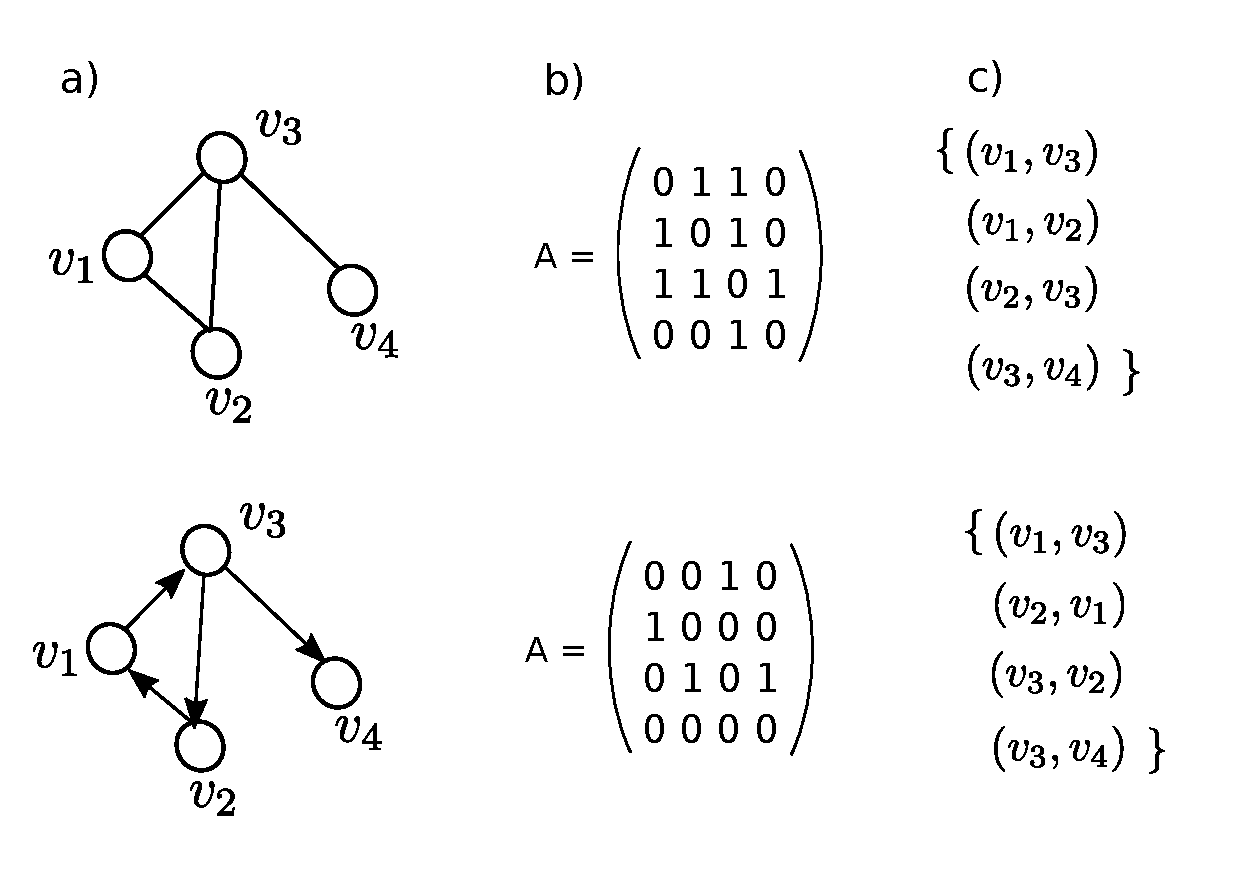
\includegraphics[width=0.7\linewidth]{directed_graph.pdf} 
	\caption[Graph, matrix and edge list representations.]{a) Graph representation of undirected (top panel) and directed (bottom panel) network. The same networks are represented with adjacency matrices column b), and edge list representation in column c).}
	\label{fig:graph_dir}
\end{figure}

The number of edges and nodes are dependent variables. Considering that each node can make $N-1$ connections, the maximum number of the edges in the network is $L_{max}=N(N-1)/2$, as each edge is counted twice. For directed network it is possible to draw $L_{max}=N(N-1)$ edges \cite{caldarelli2007scalefree}. When it comes to large networks, they are sparse, meaning that the number of links is $L<<L_{max}$. As consequence, the adjacency matrix is also sparse structure (has many zeros) that takes large portion of computer memory \cite{barabasi2016network}. 
It is common to represent the graph as edge list. In this case, illustrated on Figure \ref{fig:graph_dir}, column c), graph is described with the list of links that are in the graph, $G = \{ \{v_i,v_j\}\}$. Still with this representation we are not able to distinguish between directed and undirected graph structures, so in the computational algorithm should be specified if the edges are considered symetric or not.  


\begin{figure}[h]
	\centering
	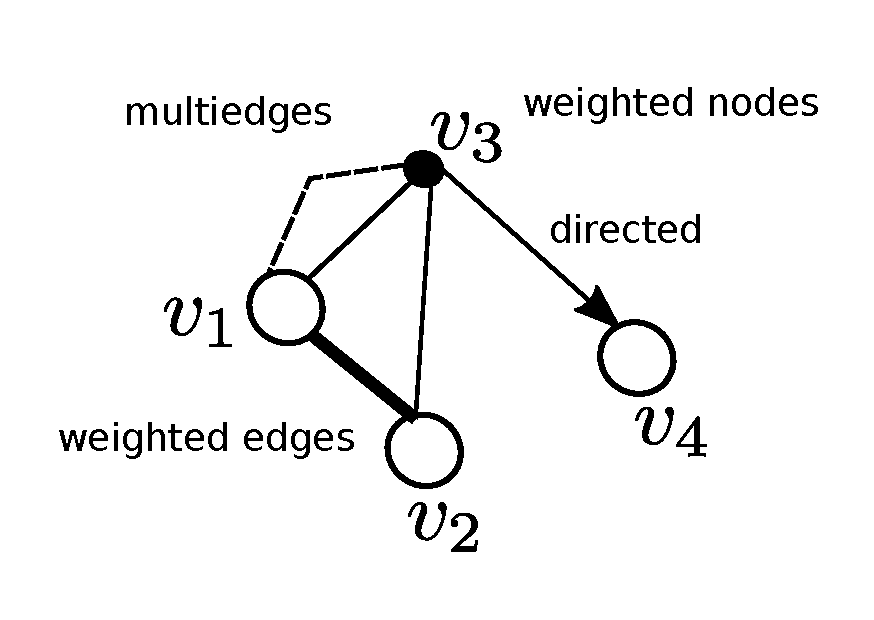
\includegraphics[width=0.4\linewidth]{multi_graph.pdf} 
	\caption[Different network representations.]{The complex networks may represent different characteristics of the system. The edges can be directed, weighted or multiply. Also nodes can be assigned with different weights or any relevant feature.}
	\label{fig:multigraph}
\end{figure}

Sometimes is essential to include the specific properties of the system in the network representation. For example, to emphasis the frequent interactions between nodes, edges can be assigned with different values, such networks are \textbf{weighted}. They can be described with adjacency matrix, whose elements can take any real number $A_{ij}=w_{ij}$ and $w_{ij}>0$. In general edges may be associated with any categorical variable. Similarly additional properties can be added to nodes, or even to the whole network structure. To include the \textbf{temporal} component in the network, edges are characterized with the time when the interaction between nodes happen. Finally, if two nodes interact in different ways, the \textbf{multigraph} is appropriate configuration where multiply edges are allowed. The graphical representation of discussed network representations is given on the Figure \ref{fig:multigraph}.

A \textbf{bipartite network} consists of two types nodes. The nodes in the same partition are not connected, while links exist only between partitions. For many real systems, a bipartite graph is a natural representation\cite{barabasi2016network, latora2017complex}. For example, the bipartite network of people and groups has two distinct node partitions while links indicate the memberships. Another example is a system of customers and products. The link between user and item is created when the user buys an item. The bipartite networks find their application in the algorithms for recommended systems, whose goal is to recommend items that may interest the user. Actually, to find the most probable missing links in the network. 

In a bipartite network, nodes in one partition are not connected. Still, we can analyse a single node type if we project the bipartite network on one partition. The primary assumption is that two nodes in one partition could be connected if they point to the same node in another partition. Consider the network of movies and actors. The one mode projection of movies is an undirected network whose links indicate that two movies share the same actors. On the other hand, another projection is a network of actors. The links exist if two actors appear in the same movie \cite{newman2010, barabasi2016network}.

\begin{figure}[h]
	\centering
	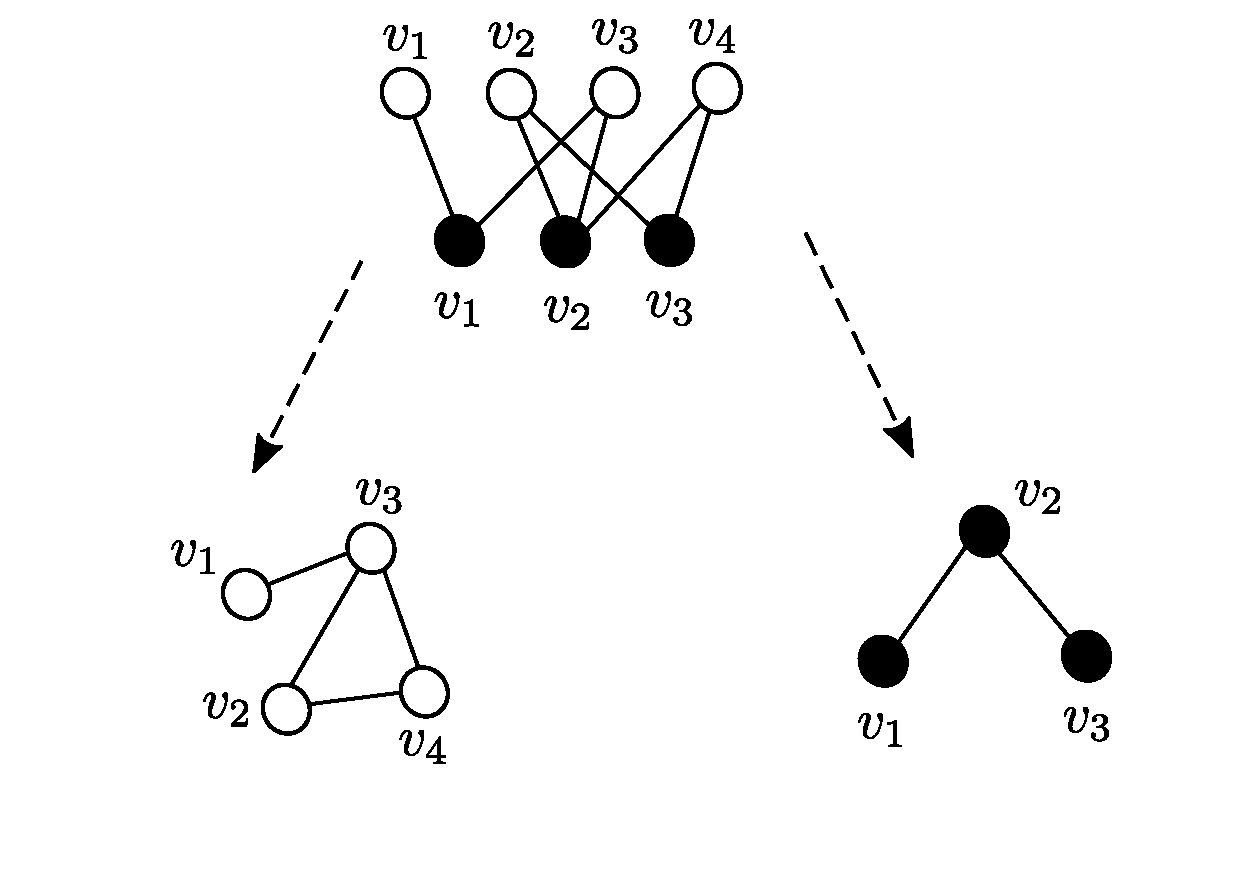
\includegraphics[width=0.7\linewidth]{bipartite_graph.pdf} 
	\caption[Bipartite network.]{Bipartite network and two partition projections.}
	\label{fig:gt2}
\end{figure}

We should be aware that important information is lost when creating a one-mode projection. First of all, without having weighted edges in the network of actors, it is impossible to have information on how many movies two actors appear in. From the one-mode projection, we can not reconstruct the original network. Moreover, two different bipartite networks may have the same projected networks. The important consequence of the network projection is the creation of cliques; subgraphs where all nodes are connected. \\
In general, it is possible to define the k-bipartite network. The same rules apply as before. There are $k$ distinct node partitions, while the edges exist only between different types of nodes.

\textbf{Temporal networks.}
Studying the real systems as static networks can give us a lot of insight into the system properties. Still, real systems are not static; they evolve not only in the number of elements but also in the number of interactions between them. Some interactions in the system may repeat in different intervals and could be described with complex activity patterns. Including time dimension in the network representation allows us to study the properties of the system closely. The temporal information may matter a lot \cite{holme2012}. For example if interaction between nodes $(v_1, v_2)$ happened before in time than  $(v_2, v_3)$, then nodes $v_1, v_3$ would not be connected, as it is the case in the static network. 

The temporal network is a collection of timestamped edges. Each edge is defined as $(v_i, v_j, t, \Delta t)$, where $v_i$ and $v_j$, are nodes $t$ is time when interaction happen, and $\Delta t$ is event duration \cite{guide_temporal}. The duration of the events may vary, as in the phone-call network. Also, for many systems, the time resolution of event duration is too small. For example, this parameter may be neglected when people interact on social platforms or email each other because the event time is too short, it scales in seconds.

\begin{figure}[h]
	\centering
	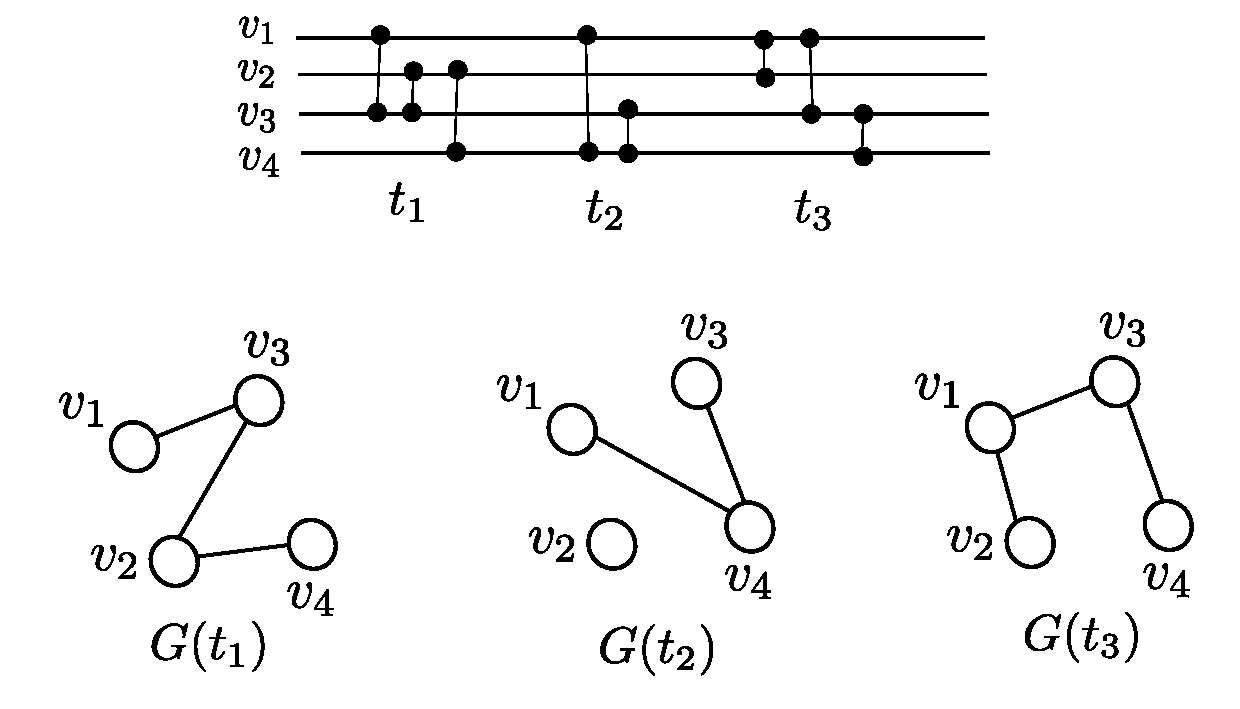
\includegraphics[width=0.7\linewidth]{temporal_network.pdf} 
	\caption[Temporal network.]{Temporal network. }
	\label{fig:gt3}
\end{figure}

The temporal network can be represented as sequence of static networks that evolve in time, $G = \{ G(t_1), G(t_2), ..., G(t_{max})\}$. At each time step, we can create the network and analyze the macroscopic properties of the given network snapshot. With this, we can end up with graph snapshots with many disconnected components or empty graphs for some points \cite{holme2015modern}. Sometimes, a much better approach is to aggregate the links that over time-windows. Here, we need to specify the time window length $w$. Interactions in the time interval $0\leq t<w$ enter the first snapshot. The next snapshot takes edges $w \leq t <2w$, and so on. The time windows are not overlapping, but generally, it is possible to slide the time window for different periods $ 1 \leq \delta t \geq w$. The downside of this method is that we can not recover original data points. The larger the time window is, the more information is lost. If the time window is set to $w=t_{max}$, there is only one snapshot, and the temporal data are no more available \cite{krings2012effects, arnold2021moving}. 

\textbf{Multilayer networks} were introduced for studying systems in which different types of interaction exist. This formalism allows one to investigate diverse network systems and to combine different types of data into one model \cite{porter2018multilayer}. In a multilayer or multiplex network, all nodes are present in each layer, but their interactions among layers differ. Two nodes may be connected in one layer but not in the other. Different online social systems may be an example of a multiplex network when users are connected on one platform but not on the other \cite{aleta2019multilayer}. Or the airline transportation network, where each layer represents the flights of different airline companies \cite{kivelamultilayer}.   

\section{In this thesis}

In this thesis we use statistical physics and complex network approaches to model and empirically analyze online social systems. These systems consist of many users interacting in various ways on online platforms and could be represented by complex networks. In chapter \ref{Ch:Method}, we provide the methodology employed for this research. We describe the fundamental measures of complex networks and introduce basic complex network models. Section 2.5 reviews the most common probability distributions that characterize the properties of complex systems and outlines distributions fitting methods. Finally, we introduce the multifractality of the time-series and dynamical reputation model. 

The chapter \ref{Ch:signals} addresses the difference between network models where the growth in a number of nodes is constant and when it follows a non-trivial growth signal. This research aims to quantify how growth signals influence the structure of complex networks. Using the adapted ageing model \cite{hajra2004}, we use computer simulations to generate different kinds of complex networks. For more realistic real-world network simulations, growing signals are time series of new users from online social platforms, MySpace and Tech group from Meetup. They are described with trends, cycles and long-range correlations. Often time-series have multi fractal properties. The results of this study are published in \cite{vranic2021growth}, and they show the importance of growth signals in shaping the network structure because the scale-free networks, which represent real systems, are mainly altered. 

As research on social groups mainly focuses on a single group, there are remaining questions about the characteristics of the entire system. 
%It has been shown that the distribution of company sizes follows log-normal behaviour and remains stable over decades \cite{stanley1996scaling}, and similar results are found for the sizes of cities \cite{barthelemy2016structure, barthelemy2019statistical}. 
For example, the Tech group is only one of the groups around which Meetup users organize; many other groups are created worldwide so system constantly grow. 
%So far, there has been little research on the growth of online social groups. 
In chapter \ref{Ch:Groups} we will examine how groups on online social platforms grow. The results are summarized in the paper  \cite{vranic2022universal}. This research is based on the Reddit and Meetup data. From Meetup, we create two data sets, one with groups created in London and the other with groups created in New York, while for Reddit, we selected groups built before 2012. We are interested in explaining scaling behaviour in group size distribution and growth rates of group, identifying the growth mechanisms present in the system and providing the bipartite complex network model that can reproduce the universality found in the system.

Even though across complex systems we find the emergence of universal behaviour, for example, the scaling of the degree distribution of two groups is similar, different factors might influence its success. It is well known that many online groups may suddenly fall apart. These questions are the subject of the chapter \ref{Ch:Trust}, which main results are published in the paper \cite{vranic2022sustainability}. Here, we study the question-answer platform Stack Exchange; it has more than 200 different topic-specified sites where people help each other in answering questions. What is interesting about this system is that some sites were closed because they did not produce enough activity. For that reason, we selected the sites with the same topic that failed but later, when someone proposed the site again, it stayed active. We analyze the evolution of user interaction networks, here we use the temporal network approach and compare active and closed sites. We find that it is essential how the network users are distributed into a core-periphery structure \cite{gallagher2020clarified}. The core must selects firmly connected users, but their interaction with periphery has to be high. In other words, we need a trustworthy core to hold community. Introducing the Dynamical Reputation Model (DIBRM) \cite{melnikov2018toward}, based on user interaction sequences, we quantify how much users can be trusted and whether the community has a strong core. In the appendix \ref{App:SE} we briefly describe the Stack Exchange sites, in the appendix \ref{App:parameters} and \ref{App:sliding} discuss how we choose parameters  for DIBRM model while in appendix \ref{App:robust} we discuss the stability of inferred core-periphery structures. 

Finally, in the chapter \ref{Ch:Conclussion}, we draw the main findings of this thesis. 










